\chapter{高分辨TEM图像自动表征系统}
本文的第三章和第四章着重介绍了高分辨透射显微镜的质量提升和分割方法，然而在实际应用中，单纯的图像质量提升和分割并不能满足科学家们对于原子级别信息的深入分析需求。因此，本章将重点介绍一个高分辨TEM图像自动表征系统的设计与实现，该系统旨在通过自动化的方式识别和处理原子位置，并动态提取原子细粒度信息，以支持更深入的科学研究。

\section{需求分析与系统功能设计}
\subsection{需求分析}
原子点精确识别与细粒度信息动态提取是高分辨TEM图像分析中的核心需求。科学家们需要一个能够自动识别原子位置、建立原子关系模型，并动态提取原子运动和行为特征的系统，以便更好地理解材料的结构和性能。系统需求分析主要包括以下几个方面：

（1）高分辨图像/视频自动加载与处理：系统应具备强大的数据处理能力，能够自动加载和处理高分辨TEM图像和视频数据。针对不同格式和分辨率的图像，系统应具备灵活的适应性，确保数据的高效处理和分析。在数据预处理阶段，包含多种去噪和增强算法，以提升图像质量，为后续的原子识别和分析提供更清晰的输入。

（2）原子位置识别与前景分割：系统应能够自动识别图像中的原子位置，并建立原子关系模型。这包括多原子定位、多原子关系建模以及关键参量计算，以支持后续的原子行为分析。

（3）原子细粒度信息追踪：系统应具备动态提取原子细粒度信息的能力，包括多原子运动追踪、多原子行为识别以及运动特征提取。这些功能将帮助科学家们深入分析材料的结构和性能，揭示其内在规律。

（4）用户交互与可视化：系统应提供友好的用户界面，支持用户与系统的交互操作，支持手动修改增加、删除原子点，并能够以直观的方式展示分析结果。通过可视化工具，用户可以更好地理解原子级别的信息和分析结果，从而促进科学研究的深入。

\subsection{自动化原子位置识别与处理模块}
自动化原子位置识别与处理模块主要需要为用户提供高分辨电镜图像中原子级别的精准定位与微观结构分析能力。材料研究人员通常需要处理大量高分辨透射电镜（HRTEM）等原始图像数据，这些数据往往伴随较高的背景噪声且原子衬度不一，系统最重要的功能是结合深度学习模型推理提供自动化的前景分割与原子识别能力，保证用户能够快速、低成本地从复杂图像中提取出精确的原子坐标。在识别过程中，由于不同材料的晶格结构与实际成像条件存在差异，系统还需提供完备的数据预处理（如图像去噪、原子粗分割、缩放设置）与基础计算修正功能（如邻接关系构建、异常点修改、仿射变换与夹角计算等），使得用户在模型推理前后可以灵活调整参数，并对识别出的原子阵列进行精确的人机交互校准。此外，仅获取原子坐标往往无法满足深层次的晶体学缺陷研究需求，本文系统不仅能输出基础的点位掩膜与坐标信息，还能从微观力学特征角度进行深度的应变分析（包括方向应变、面积应变和角度应变）。因此，系统开发了完善的可视化与后处理功能，支持距离与应变的直观映射、大批量数据的自动化操作以及多维度的分析信息导出。图\ref{fig:5-1}展示了自动化原子位置识别与处理模块的功能架构设计：

\begin{figure} [htb]
    \centering
    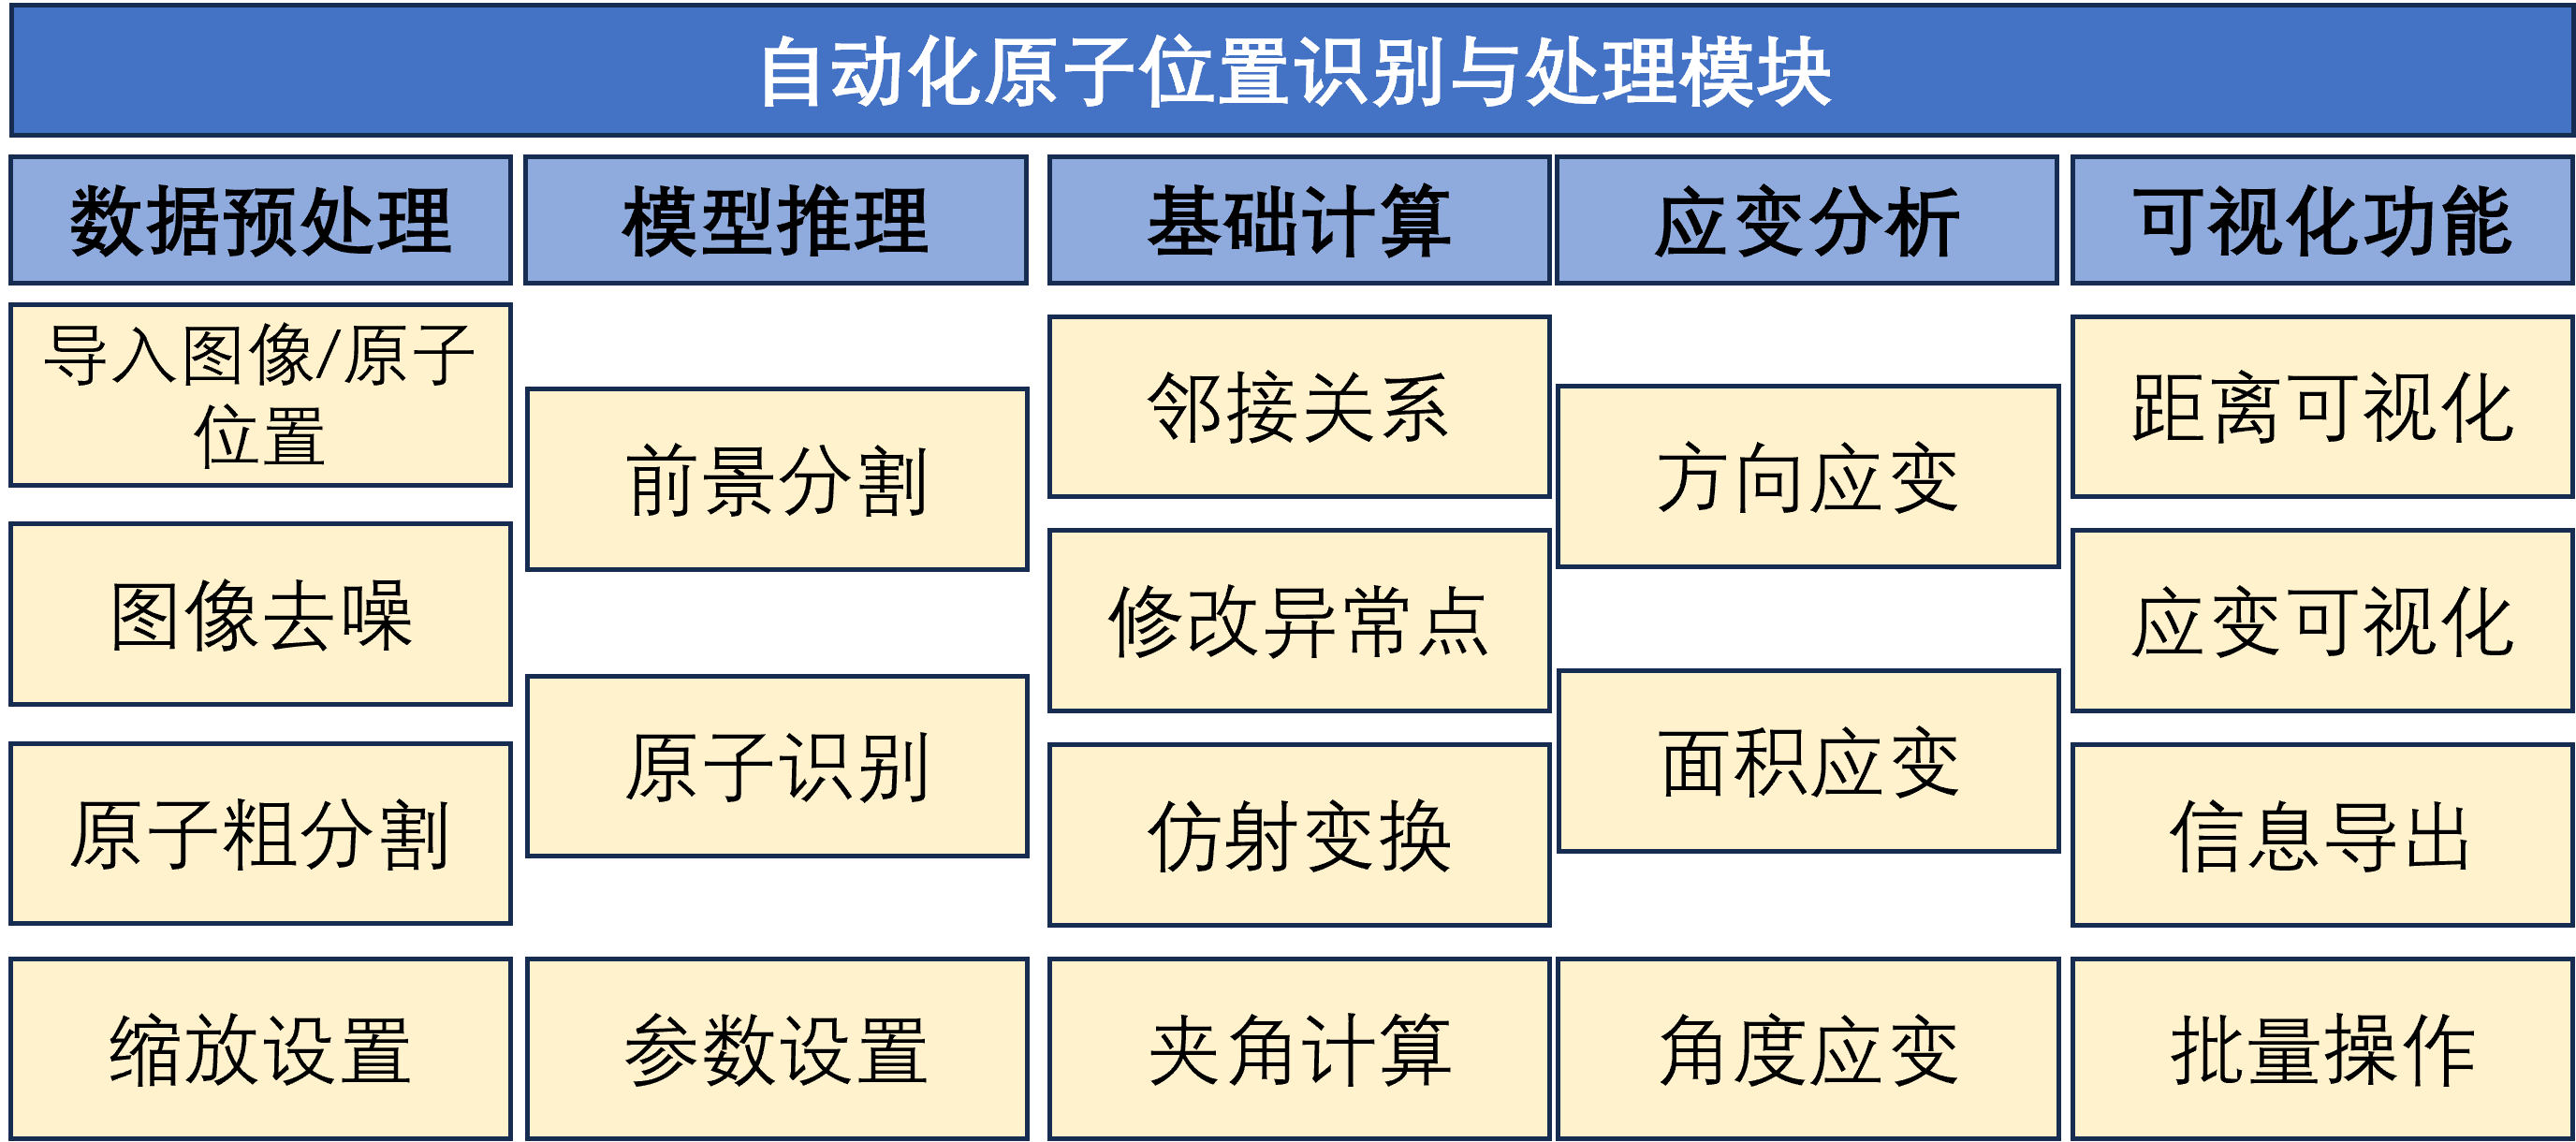
\includegraphics[width=1.0\textwidth]{images/chap5/自动化原子位置识别与处理模块.png}
    \bicaption{自动化原子位置识别与处理模块}{Automated Atomic Position Recognition and Processing Module}
    \label{fig:5-1}
\end{figure}

\subsection{原子细粒度信息动态提取模块}
原子细粒度信息动态提取模块主要需要为用户提供原位电镜视频序列中原子级别的动态追踪与细粒度行为分析能力。材料研究人员通常需要处理大量的原位动态观测视频数据，这些数据往往伴随不可避免的样品整体漂移且包含成百上千的连续帧，系统最重要的功能是结合自动漂移校正与DBSCAN聚类算法提供高鲁棒性的运动追踪能力，保证用户能够快速、准确地从连续视频帧中提取出原子的动态演变轨迹。在追踪分析前，由于原始视频往往冗长且包含非关键片段，系统还需提供完备的视频处理功能（如帧率调节、片段截取与视频帧导出），使得用户可以灵活地对原始视频进行预处理，聚焦于关键的反应阶段。此外，仅获取原子的整体运动轨迹往往无法满足对特定催化反应或局部结构演变的深层次研究需求，本文系统不仅能输出基础的轨迹坐标，还能针对特定区域进行活性位点分析，并提取多维度的细粒度特征（如特定方向的位移与角度变化）。因此，系统开发了完善的辅助与后处理功能，支持轨迹信息的交互式查询联动、大批量追踪结果的结果多维导出以及表征数据的独立保存。图\ref{fig:5-2}展示了原子细粒度信息动态提取模块的功能架构设计：

\begin{figure} [htb]
    \centering
    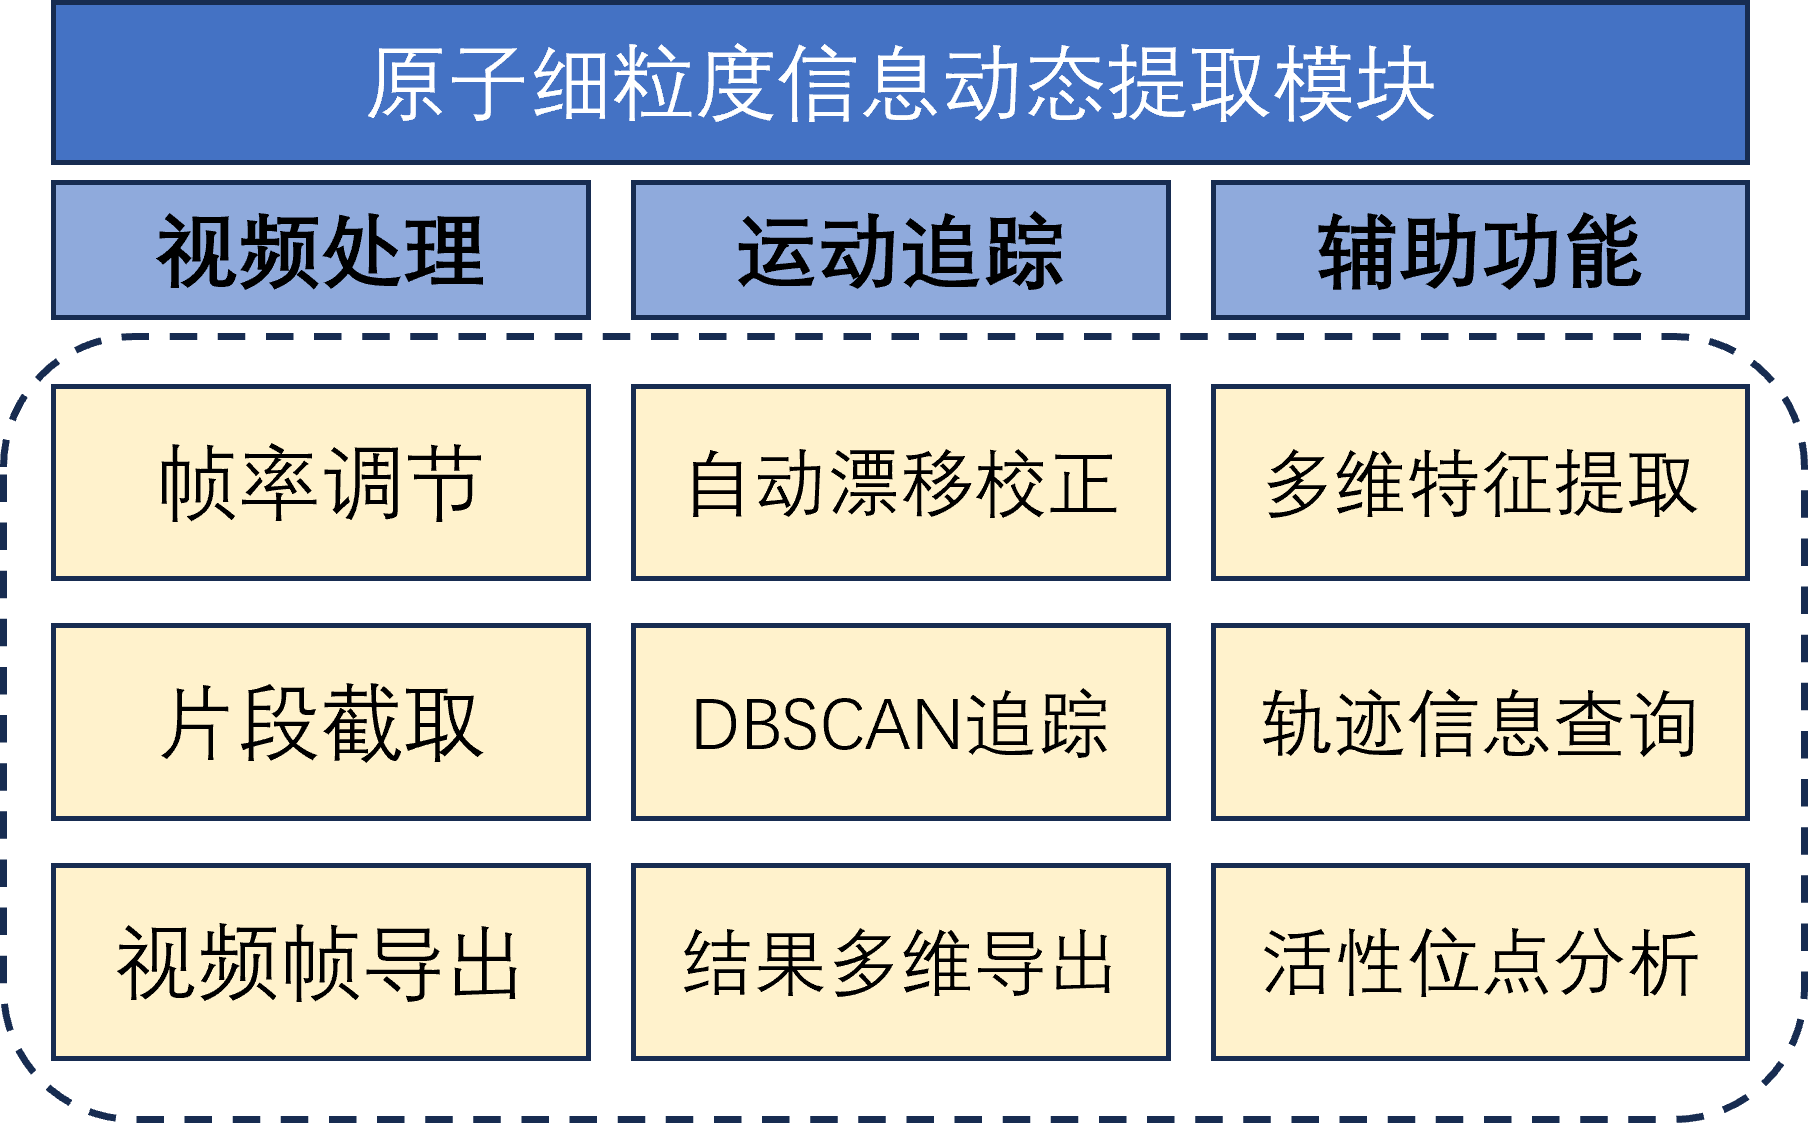
\includegraphics[width=0.8\textwidth]{images/chap5/原子细粒度信息动态提取模块.png}
    \bicaption{原子细粒度信息动态提取模块}{Atomic Fine-grained Information Dynamic Extraction Module}
    \label{fig:5-2}
\end{figure}

\section{总体架构设计}
根据上一节的需求分析与功能描述，对系统进行两个模块的架构设计，并且对子功能模块进行了层次划分。系统的总体架构设计如图\ref{fig:5-3}所示：

\begin{figure} [htb]
    \centering
    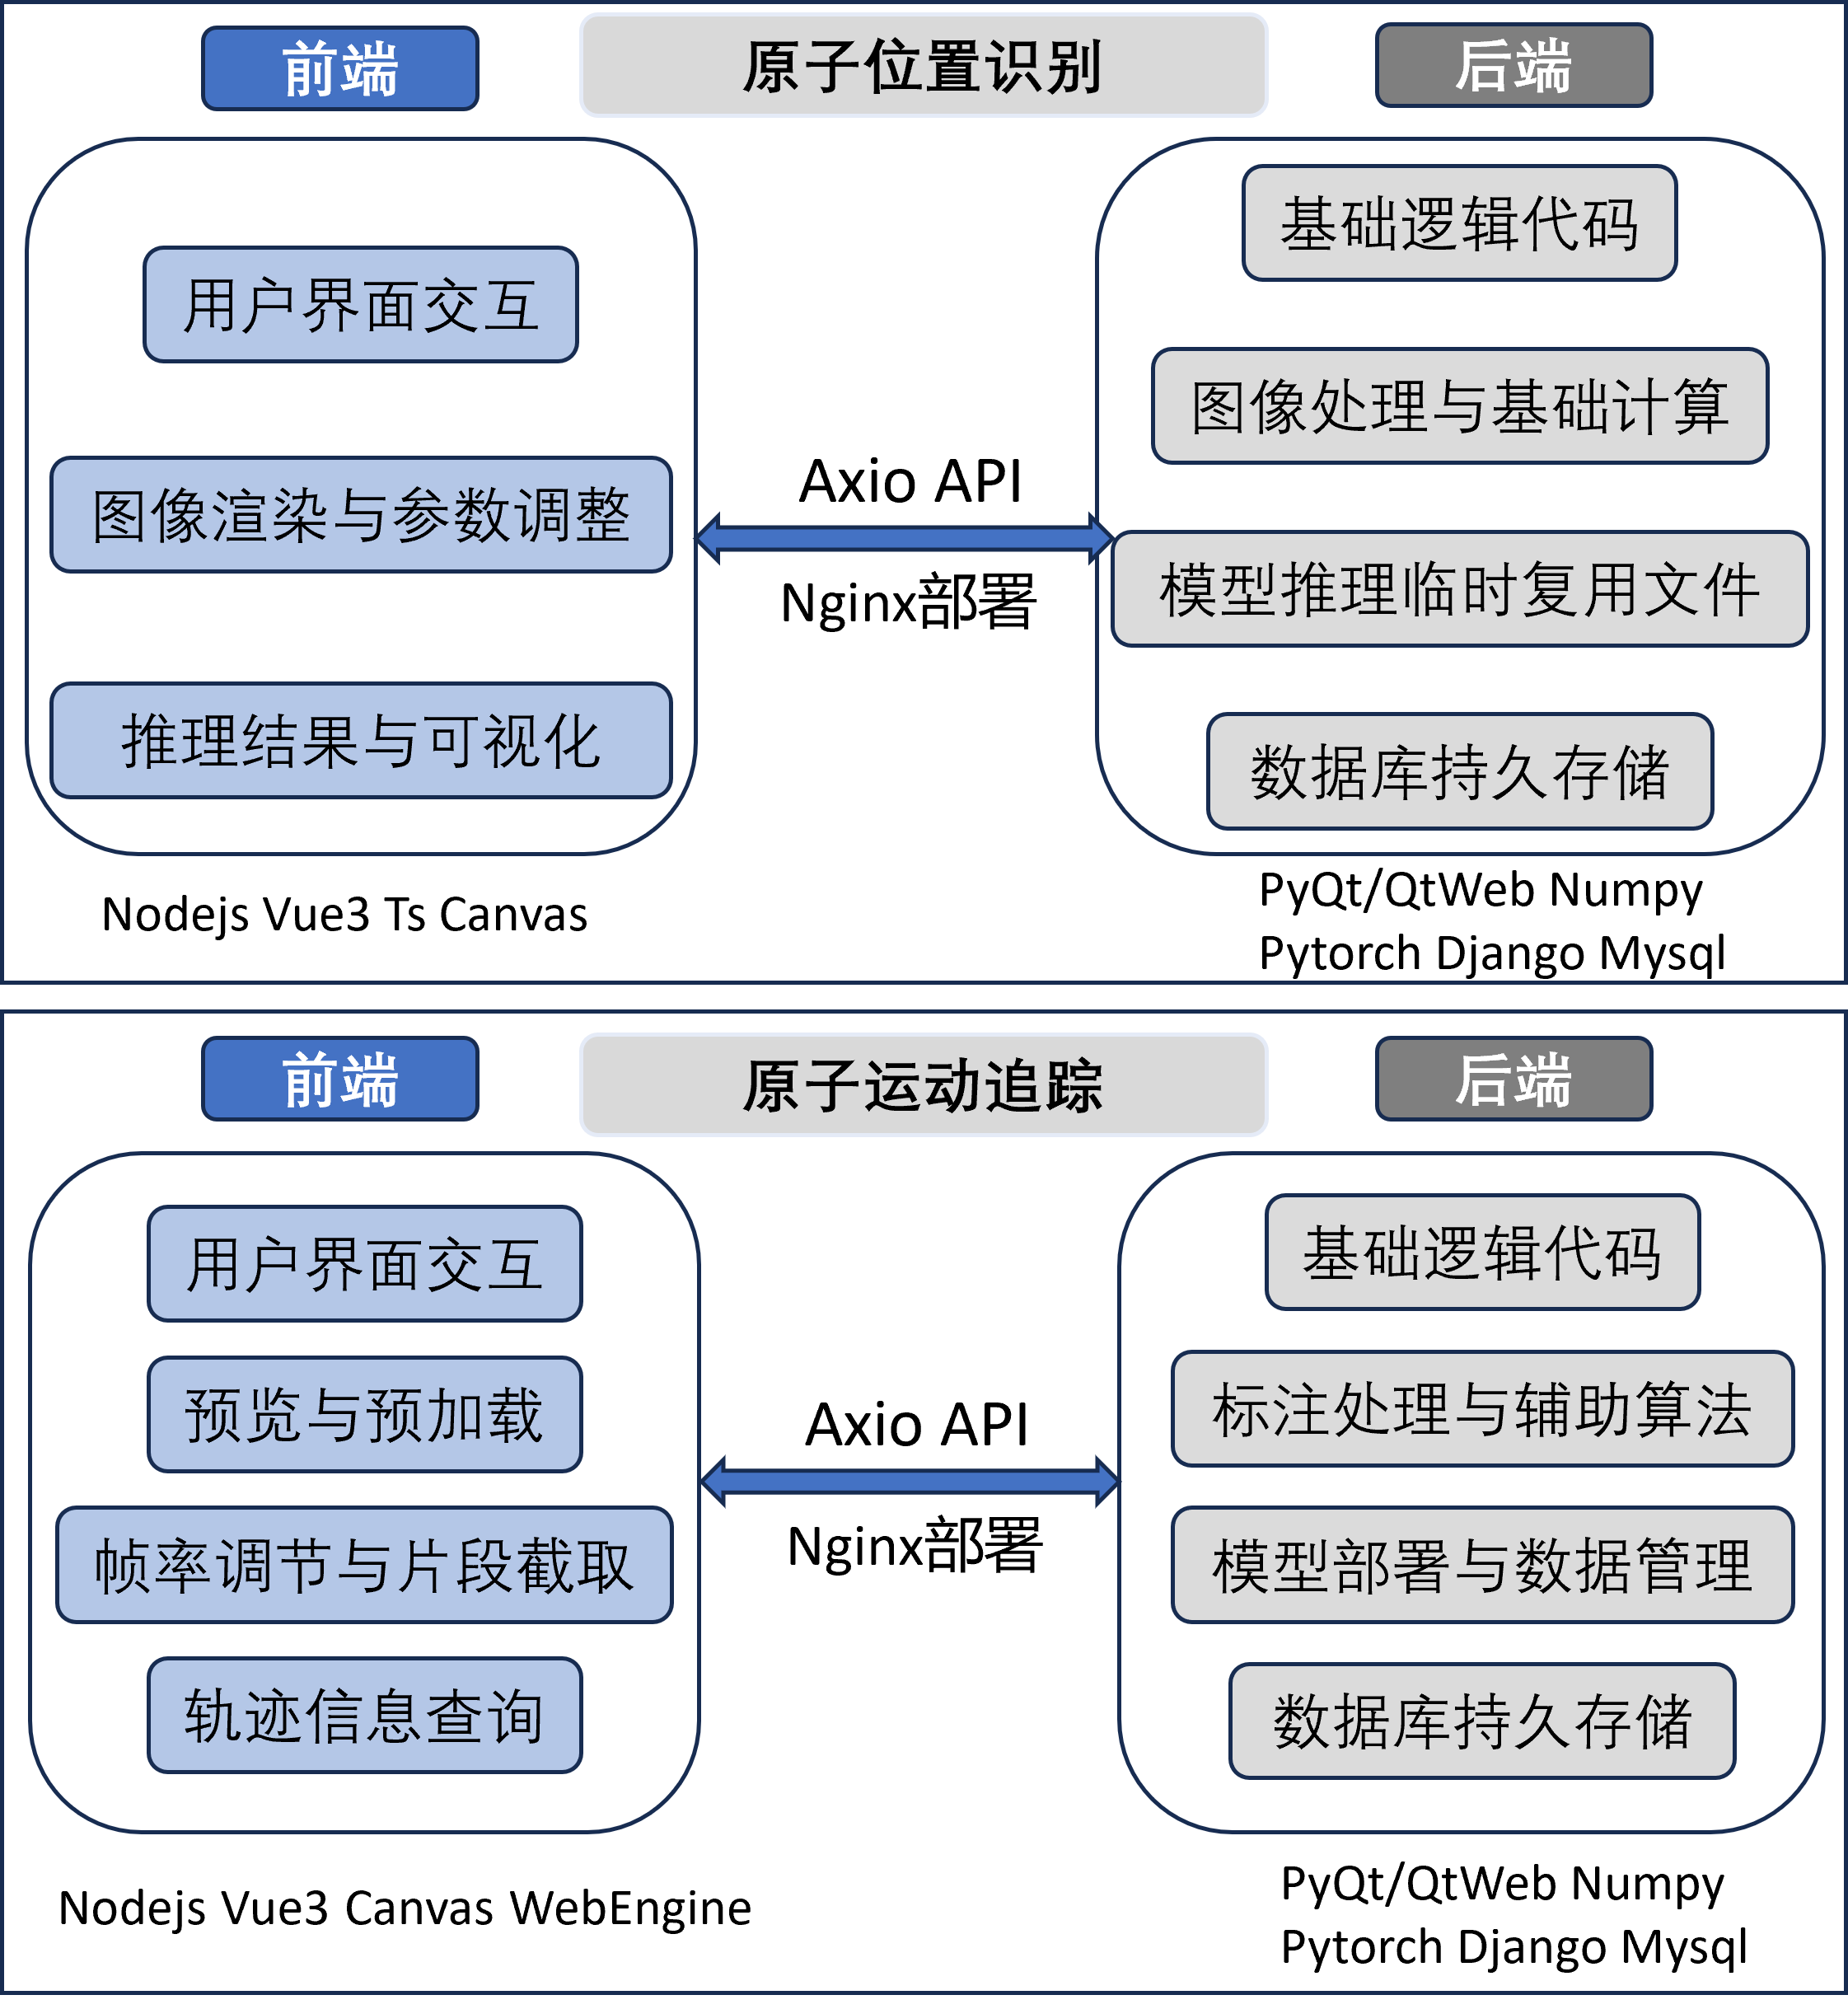
\includegraphics[width=1.0\textwidth]{images/chap5/系统总体架构设计图.png}
    \bicaption{系统总体架构设计}{Overall System Architecture Design}
    \label{fig:5-3}
\end{figure}

原子位置识别模块包含前后端两个主要部分，其中前端包括用户交互主界面，包括图像展示、参数设置区、模型使用、信息输入等界面；图像渲染与参数调整，通过js动态加在与存储逻辑在前端实现快速的图像结果更新和超参数传递功能；推理结果与可视化，在前端进行额外存储，提升系统响应能力。前端选型Nodejs、Vue3以及TypeScript和Canvas技术实现。后端包括基础逻辑代码实现，处理模型输入输出、前后端交互接口以及数据管理等功能；图像处理与基础计算由后端服务统一执行，主要包括图像归一化与去噪增强、分割结果后处理、原子邻接关系构建以及原子间距与夹角等关键参量计算，并通过接口将计算结果返回前端用于可视化与交互修正；模型部署在RTX4090服务器上，通过Pytorch调用，并对模型推理临时复用文件保存提升实时交互效率；底层使用Mysql数据库对图像以及操作历史等持久存储。

原子细粒度信息动态提取模块同样包含前后端两个主要部分。前端部分包括用户界面交互，负责进行视频展示以及参数设置；预览与预加载通过js动态加载与存储逻辑在前端实现快速的视频结果更新和超参数传递，提升系统响应能力；帧率调节与片段截取提供用户对原始视频的灵活预处理功能，支持用户聚焦于关键反应阶段；轨迹信息查询与联动通过前端实现交互式查询与结果联动，支持用户对追踪结果的深入分析。前端技术选型为Nodejs、Vue3以及Canvas和WebEngine技术。后端部分包括基础逻辑代码，处理视频和对应的原子位置；标注处理与辅助算法负责检查文件格式不正确或是否缺少必需的列，利用Numpy和OpenCV等库进行视频帧率调节、片段截取以及自动漂移校正等预处理操作；数据库持久存储，使用Mysql数据库对追踪结果和操作历史进行持久化存储。

\section{详细设计与实现}
本节对需求分析部分整理的系统模块与功能进行详细技术实现与系统展示。本节中，分别介绍高效分割与提取模块和一体化校正标注模块的技术实现，并对重点技术进行细致描述。
\subsection{系统技术选型}
如上一节系统总体架构所述，本文构建的原子结构智能分析系统主要面向材料显微图像与原子运动视频的自动化分析场景，需要兼顾高效计算能力、良好的用户交互体验以及系统的可扩展性与可部署性。因此，本文在系统设计过程中采用前后端分离的Web架构。前端主要负责用户界面展示与交互逻辑实现，后端负责算法计算、模型推理以及数据管理。该架构能够降低系统耦合度，提升系统维护性，同时便于后续功能扩展与部署迁移。

在前端技术选型方面，系统采用Node.js运行环境与Vue3框架构建Web界面，并结合TypeScript提升代码可维护性；图像与轨迹可视化采用Canvas完成二维渲染。针对高精度标注与动态可视化的桌面端需求，本文对Python GUI方案进行了比较：Tkinter与wxPython可满足基础功能，但在组件生态与渲染能力方面存在不足；因此最终选用PyQt，依托Qt组件体系与OpenGL集成能力支持多视图同步渲染和标注工具链开发。在后端技术选型方面，系统采用Python实现核心业务逻辑，结合PyTorch完成模型加载与推理，并通过API接口实现前后端数据交互与任务调度。在数据存储方面，系统采用MySQL对图像、视频及推理结果等数据进行统一管理与持久化存储，以满足系统的查询与管理需求。

综上所述，系统最终形成了以Node.js、Vue3与Canvas为核心的Web前端交互框架，并在高精度桌面交互场景中采用PyQt扩展可视化能力；后端以Python与PyTorch为核心完成计算与推理，并结合MySQL数据库实现数据管理的整体技术体系，在保证系统计算效率的同时提供良好的交互体验与可扩展性。

\subsection{自动化原子位置识别与处理模块实现}
本节在系统架构基础上，融合了本文第四章提出的原子定位方法，允许用户进行高精度的原子位置识别并进行相关表征处理。

\textbf{(1)图像上传与预处理：}

本系统基于Web端开发，图\ref{fig:5-4}展示了系统中上传图像堵塞过程。用户可以在系统中选择待处理图像，并通过鼠标进行自动缩放和预览。系统支持多种图像格式的上传，并支持显示原图、图像复原、显示尖峰、显示编号等预览模式。

\begin{figure} [htb]
    \centering
    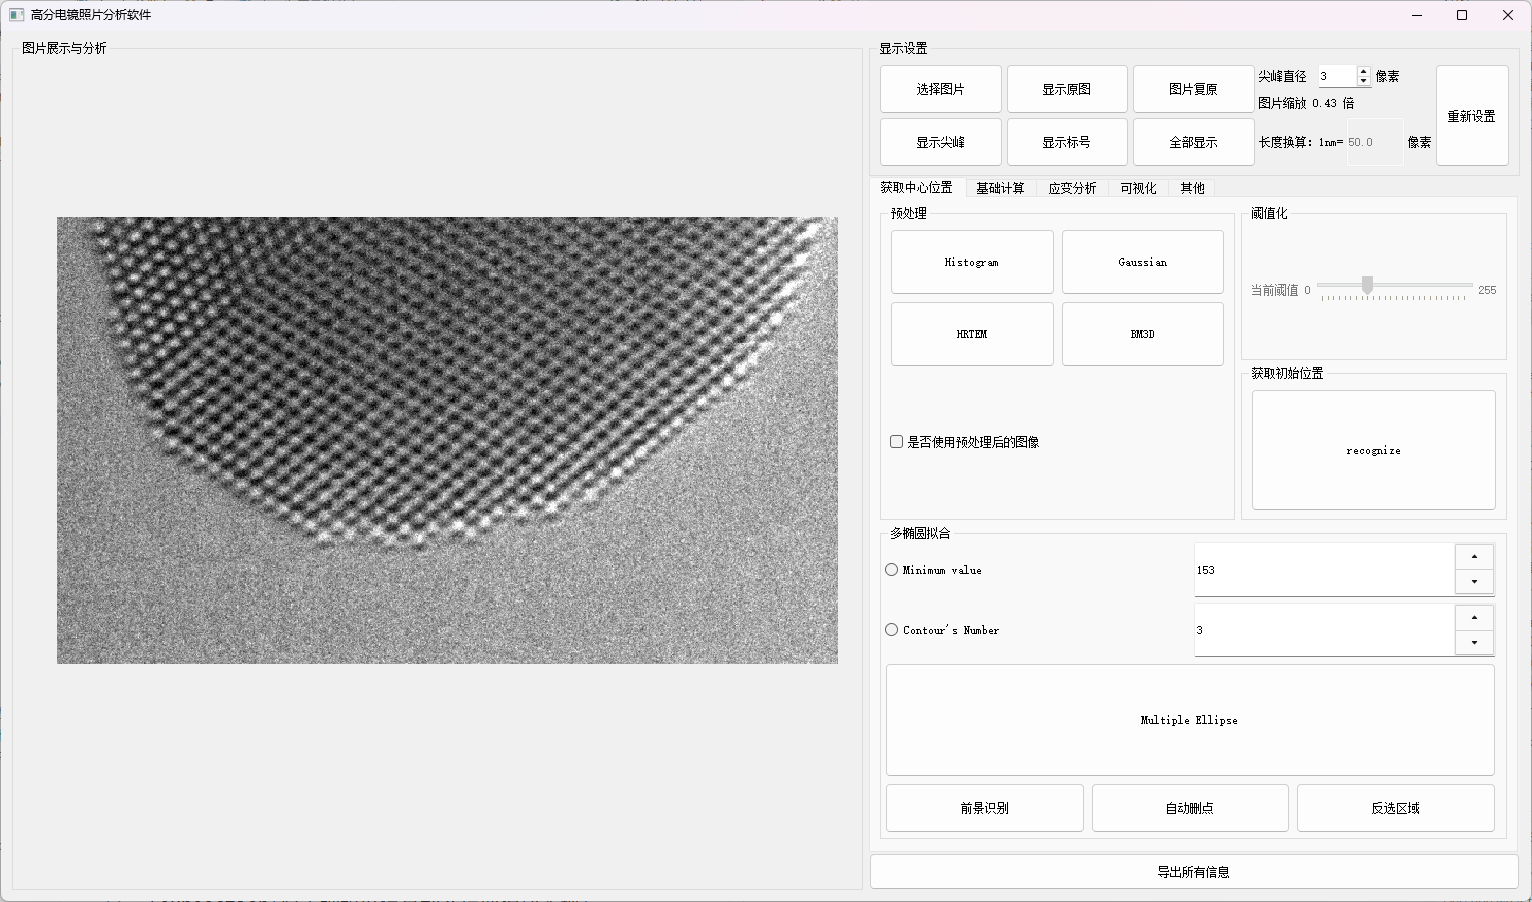
\includegraphics[width=0.8\textwidth]{images/chap5/图像上传.png}
    \bicaption{TEM图像上传与预览}{TEM Image Upload and Preview}
    \label{fig:5-4}
\end{figure}

在图像预处理阶段，用户可以选择不同的去噪算法：如直方图均衡化、高斯滤波、HRTEM滤波、BM3D滤波，如图\ref{fig:5-5}所示，该功能支持参数自定义，用户可以根据实际情况对预设的参数进行修改。如果用户对预处理结果不满意，可以通过图像复原的功能将图像恢复到原始状态，重新选择去噪算法和参数进行处理。通过这些预处理功能，用户可以提升图像质量，为后续的原子位置识别提供更清晰的输入数据，从而提高识别的准确性和鲁棒性。

\begin{figure} [htb]
    \centering
    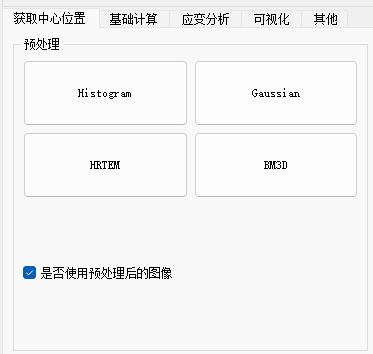
\includegraphics[width=0.6\textwidth]{images/chap5/图像滤波.png}
    \bicaption{图像滤波功能}{Image Filtering Functionality}
    \label{fig:5-5}
\end{figure}

\textbf{(2)多原子定位：}

获取原子的初始位置，首先可以通过模型推理得到原子图像的前景区域，模型推理完成后会自动在交互段显示实时的效果并存储缓存文件。如果针对某些特殊情况，原子图像的前景和背景经过设备的反色，无法正确识别出原子区域，用户可以通过反色功能将图像进行反色处理，重新进行模型推理。

前景识别完成后，用户可在前景区域内进行原子点定位。系统提供粗分割与细分割两种方式：粗分割通过灰度归一化、阈值筛选和局部极大值检测快速获得候选原子点，并经邻域合并得到初始位置；细分割则以粗定位结果为中心，在原始灰度图中截取固定窗口，采用递增阈值进行多次分割。随着阈值提高，亮斑轮廓逐步收缩，当仅保留满足条件的有效轮廓时进行椭圆拟合，提取椭圆中心并对多次结果求平均，得到最终坐标，如图\ref{fig:5-6}所示。该流程兼顾定位效率与精度，可有效降低噪声和阈值波动带来的影响。

\begin{figure} [htb]
    \centering
    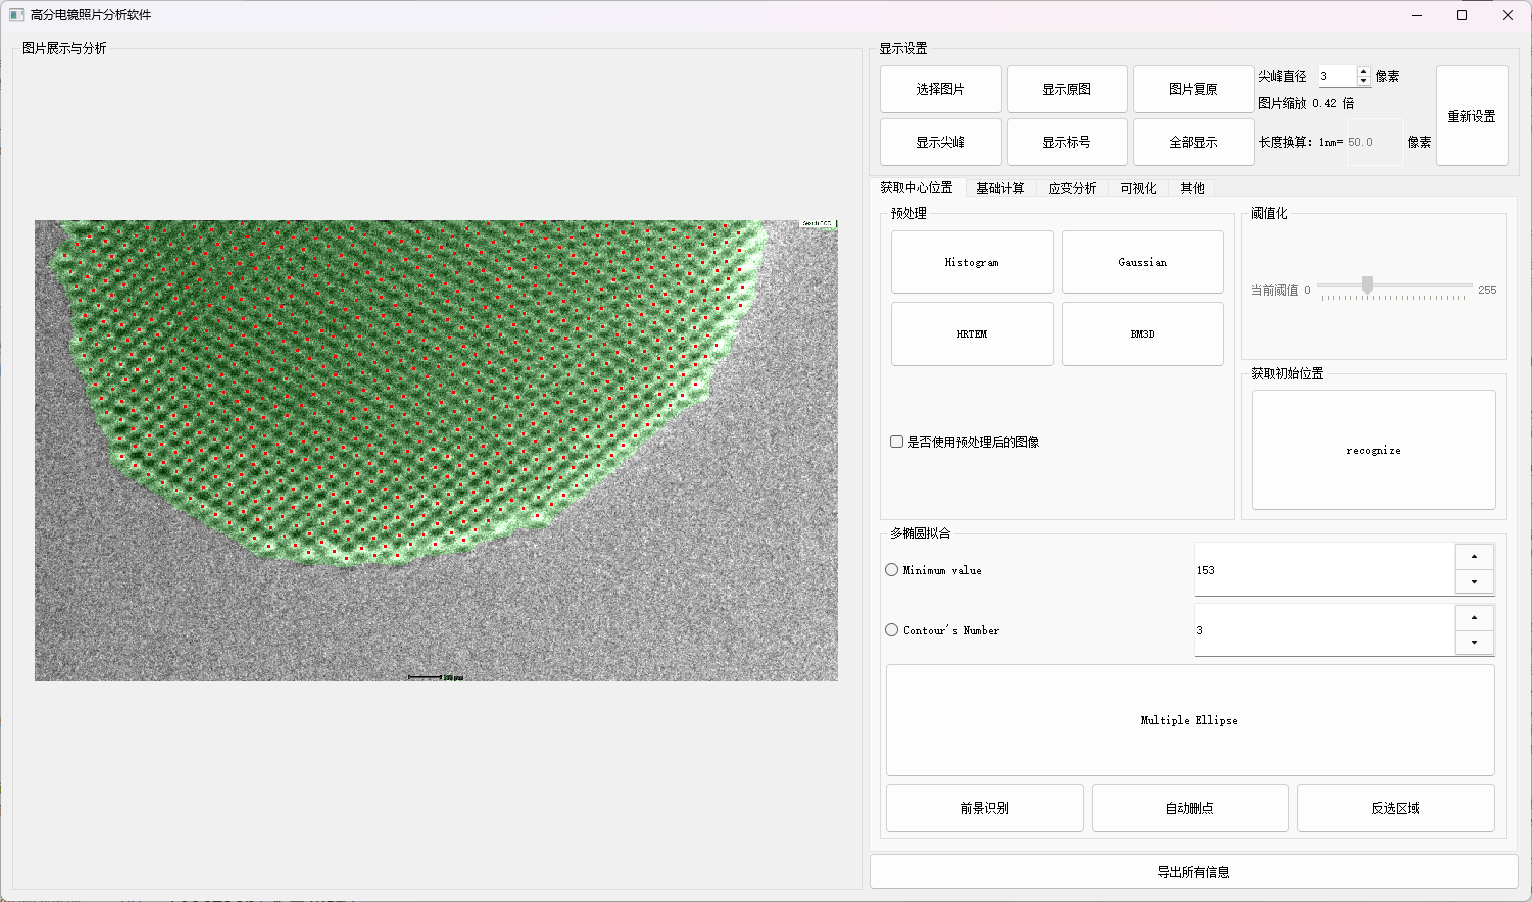
\includegraphics[width=0.8\textwidth]{images/chap5/原子定位.png}
    \bicaption{原子定位}{Atomic Positioning}
    \label{fig:5-6}
\end{figure}

\textbf{(3)多原子关系建模：}

为针对原子图像进行表征分析，系统结合原子位置识别结果，构建多原子关系模型。由于很多图像中，原子点的排列不是严格意义上符合笛卡尔直角坐标系，因此系统为用户提供了仿射变换功能，允许用户通过选择三个或更多的原子点进行仿射变换参数的计算与应用，将原子点坐标转换到一个新的坐标系中，以便更好地进行后续的分析和表征。图\ref{fig:5-7}展示了用户在图像中选取三个原子点，进行“变换结果展示”得到的矫正后的坐标系。

\begin{figure} [htb]
    \centering
    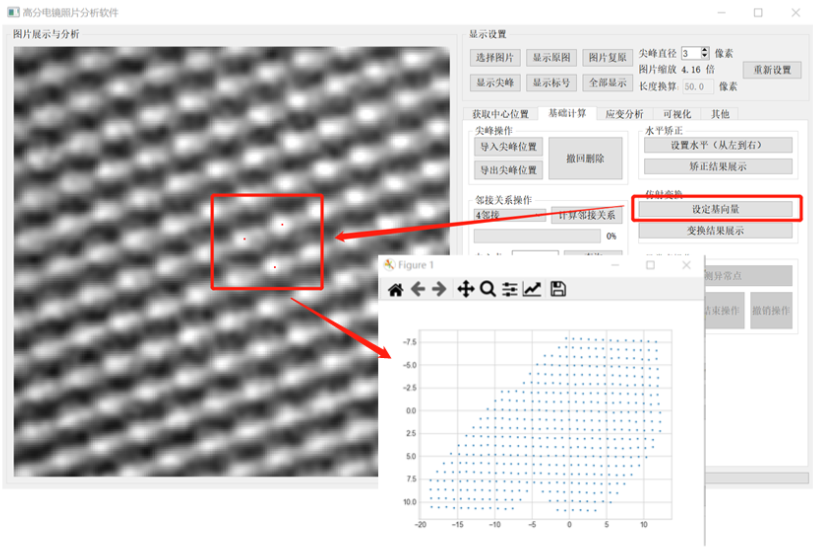
\includegraphics[width=0.8\textwidth]{images/chap5/仿射变换.png}
    \bicaption{仿射变换}{Affine Transformation}
    \label{fig:5-7}
\end{figure}

系统还提供了邻接关系构建功能，不仅可以计算单个原子点的四邻接和八邻接关系，还支持通过输入原子点标号对任意两点进行距离计算。进一步地，用户可指定任意两条边，系统基于边向量自动计算其夹角，从而满足局部构型分析与晶格几何表征需求。上述结果可与邻接关系一并图形化展示，帮助用户更直观地理解原子之间的空间关系和结构特征，如图\ref{fig:5-8}所示。此外，系统还支持异常点修改功能，允许用户对识别出的原子点进行手动修改，包括增加、删除或调整位置，以确保最终的原子关系模型准确反映实际的图像内容。

\begin{figure} [htb]
    \centering
    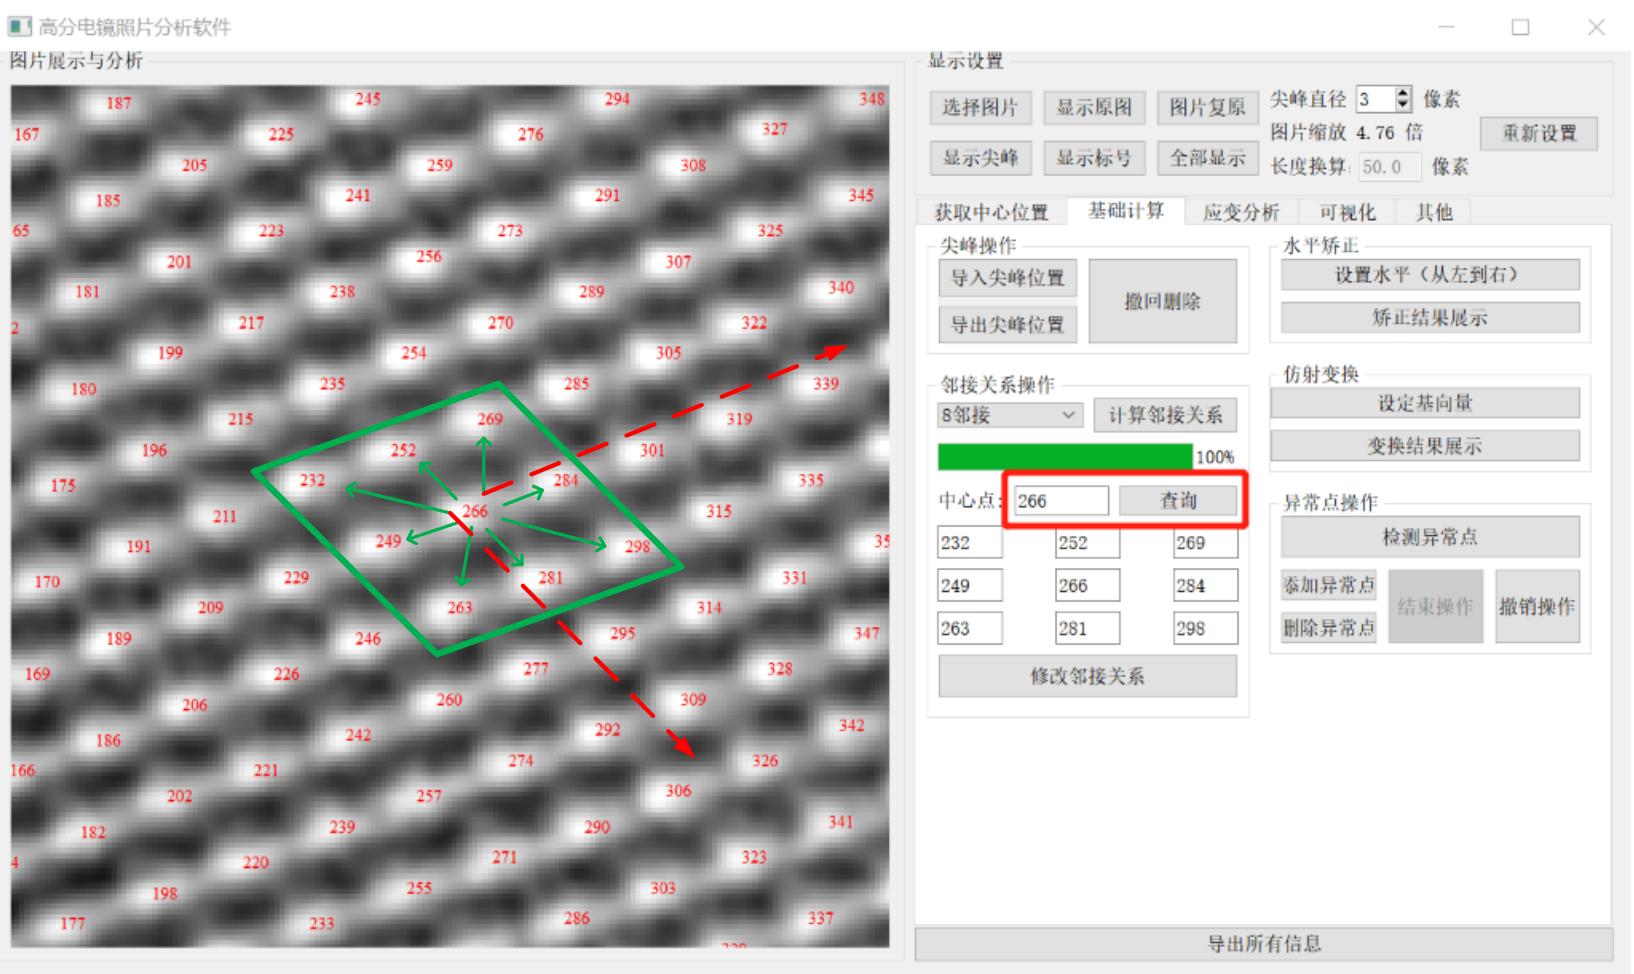
\includegraphics[width=0.8\textwidth]{images/chap5/邻接计算.png}
    \bicaption{邻接计算}{Adjacency Calculation}
    \label{fig:5-8}
\end{figure}

\textbf{(4)可视化分析与数据导出：}

为了实现对原子尺度的精确晶体学分析，系统构建了基于局部几何畸变的应变评价模型。用户可根据专业需求，针对特定晶轴方向设定参考基准值 $L_0$，系统通过计算实际原子间距 $L$ 与基准值的偏离程度；并结合夹角变化等几何特征，综合评估局部结构的应变状态，通过基于Matplotlib的可视化工具，进行图形化展示。系统支持全部信息导出为csv格式，数据样例及包含的信息如图\ref{fig:5-10}所示，每一行代表单个原子点的细粒度信息，包括八个邻接点、邻接点之间的夹角、中心点到各个邻接点之间的距离。这对详细分析材料显微图像中的局部结构和应变状态提供了重要的数据支持，并为原子细粒度追踪模块的实现奠定了基础。

% \begin{figure} [htb]
%     \centering
%     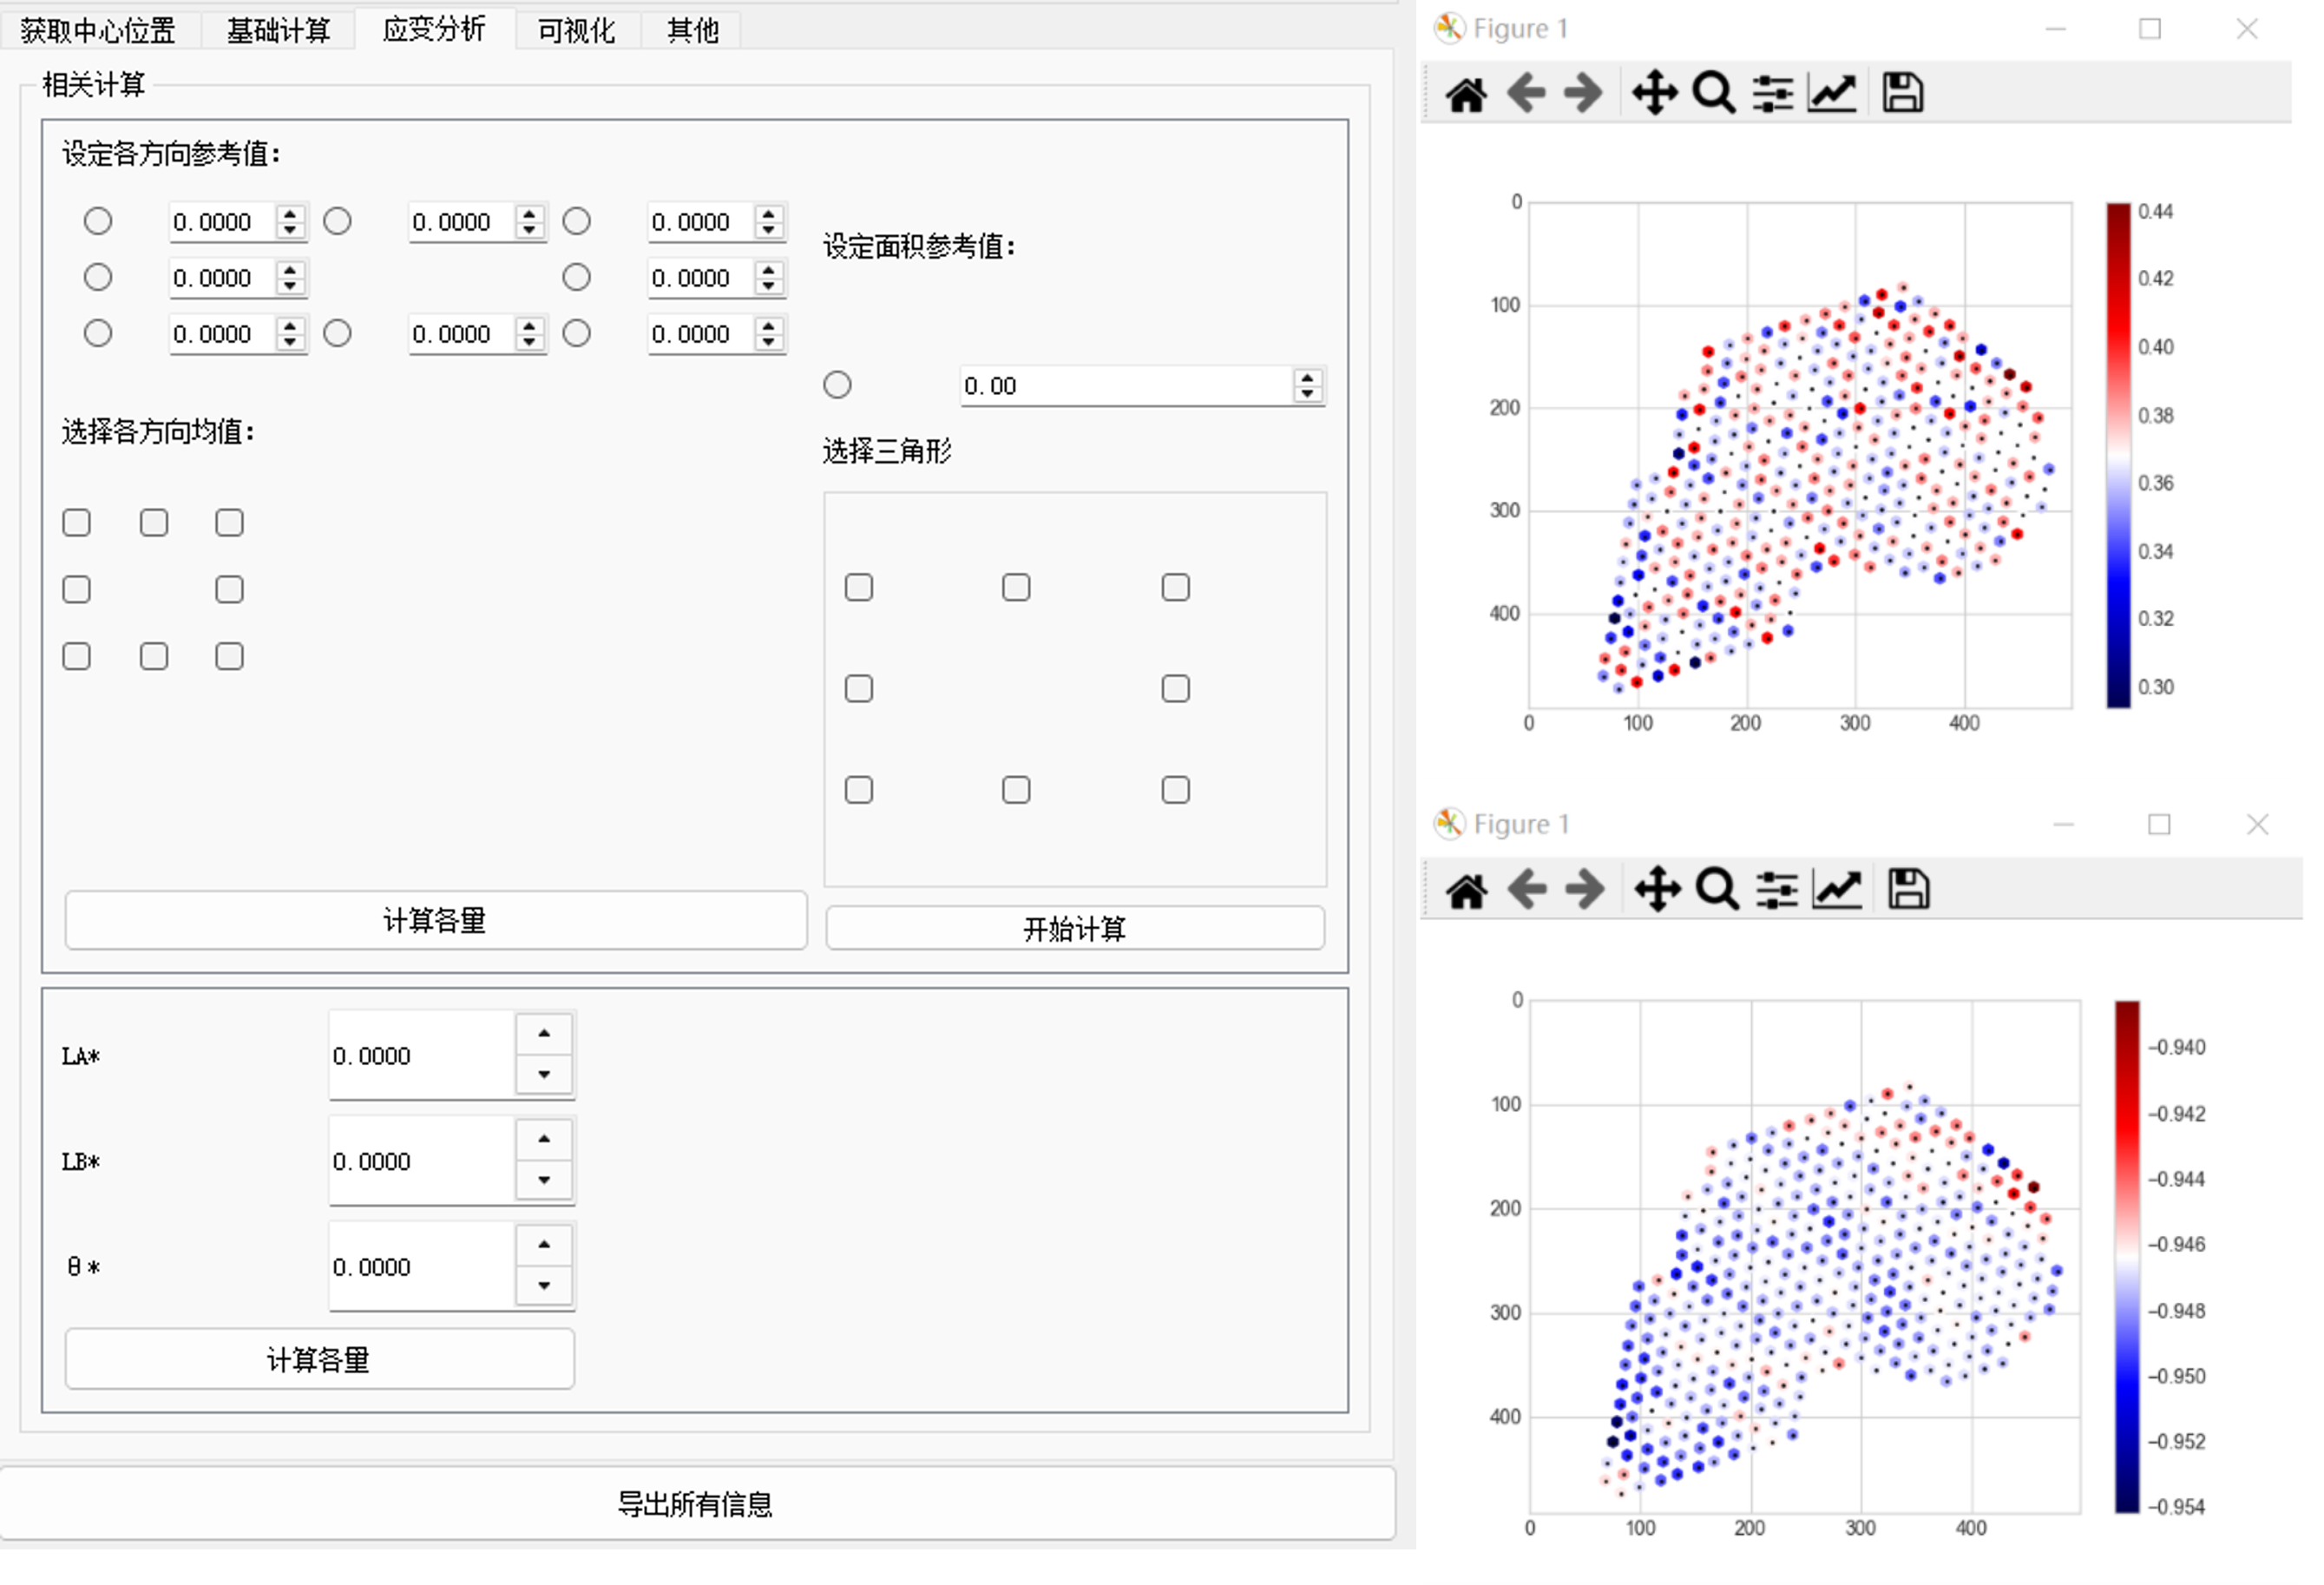
\includegraphics[width=1.0\textwidth]{images/chap5/可视化.png}
%     \bicaption{可视化}{Visualization}
%     \label{fig:5-9}
% \end{figure}

\begin{figure} [htb]
    \centering
    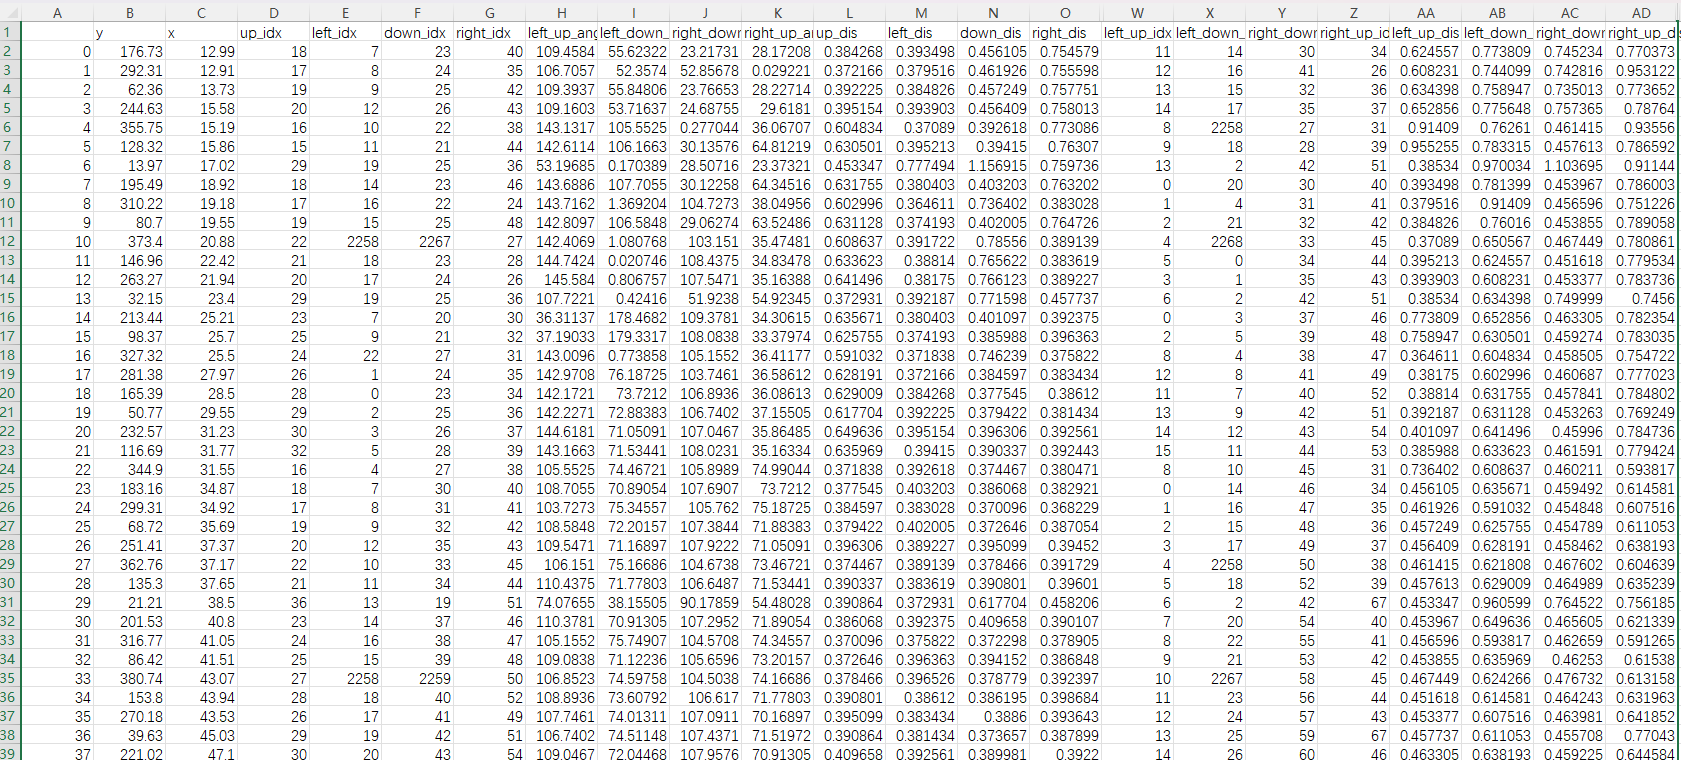
\includegraphics[width=1.0\textwidth]{images/chap5/数据导出.png}
    \bicaption{数据导出}{Data Export}
    \label{fig:5-10}
\end{figure}

\subsection{原子细粒度信息动态提取模块实现}
本节在原子定位的基础上，通过输入连续视频帧，实现对原子运动轨迹的追踪过程。系统前端采用Node.js与Vue3框架构建交互界面，通过Canvas实现轨迹的二维可视化渲染，并在桌面端场景中引入PyQt以支持多视图同步展示；后端以Python为核心语言，结合PyTorch完成行为识别模型的加载与推理，并通过MySQL数据库对追踪结果进行持久化存储。用户可以上传原位电镜视频，并自定义进行片段截取和帧率调整，将处理好的视频导出后即可进入追踪分析流程，如图\ref{fig:5-11}。

\begin{figure} [htb]
    \centering
    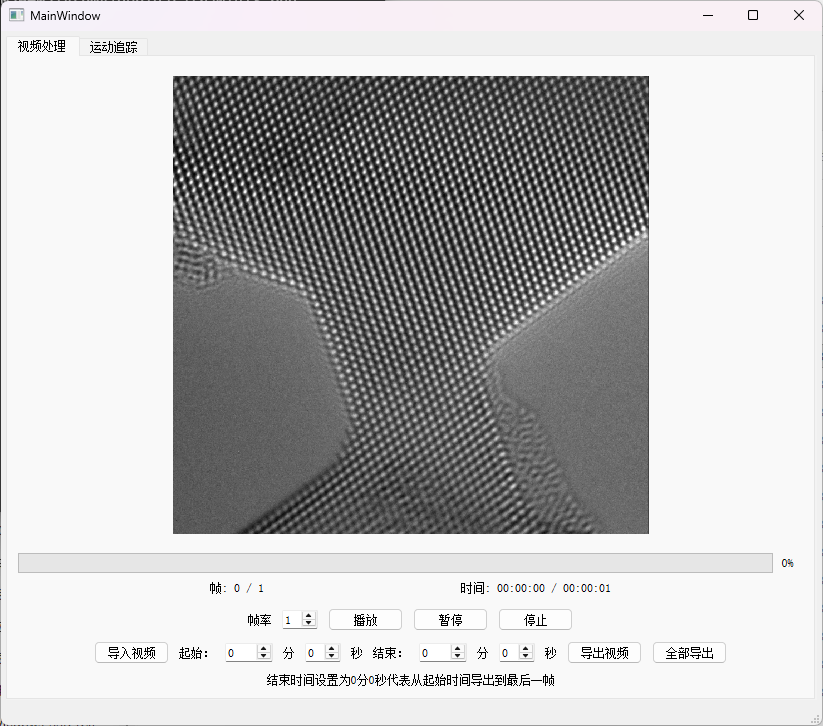
\includegraphics[width=0.6\textwidth]{images/chap5/视频上传.png}
    \bicaption{视频上传}{Video Upload}
    \label{fig:5-11}
\end{figure}

多原子运动追踪旨在从连续的视频帧中精确重构各原子的时空移动轨迹。在本节构建的系统中，用户需按顺序准备好包含原子 $x, y$ 坐标的 CSV 标准格式文件并一键上传，系统即可自动完成数据读取与校验。显示“导入成功”后即可开始追踪。系统默认漂移匹配距离为15像素、漂移最少匹配数为10帧，后端利用Numba加速算法与Numpy矩阵运算，执行复杂的自动漂移矫正以消除实验位移偏差。采用DBSCAN算法对矫正后的坐标点进行时空聚类分析，默认的追踪参数DBSCAN eps为5.0，最小样本数为10。用户可以根据实际的追踪效果进行调整，并重新执行追踪。采用默认参数对视频帧进行追踪的结果如图\ref{fig:5-12}所示。追踪完成后，可视化区域会显示所有帧的原子坐标分布的散点图，不同帧用不同颜色表示；每个追踪到的原子轨迹的聚类圆圈，圆圈半径为DBSCAN eps参数值。

\begin{figure} [htb]
    \centering
    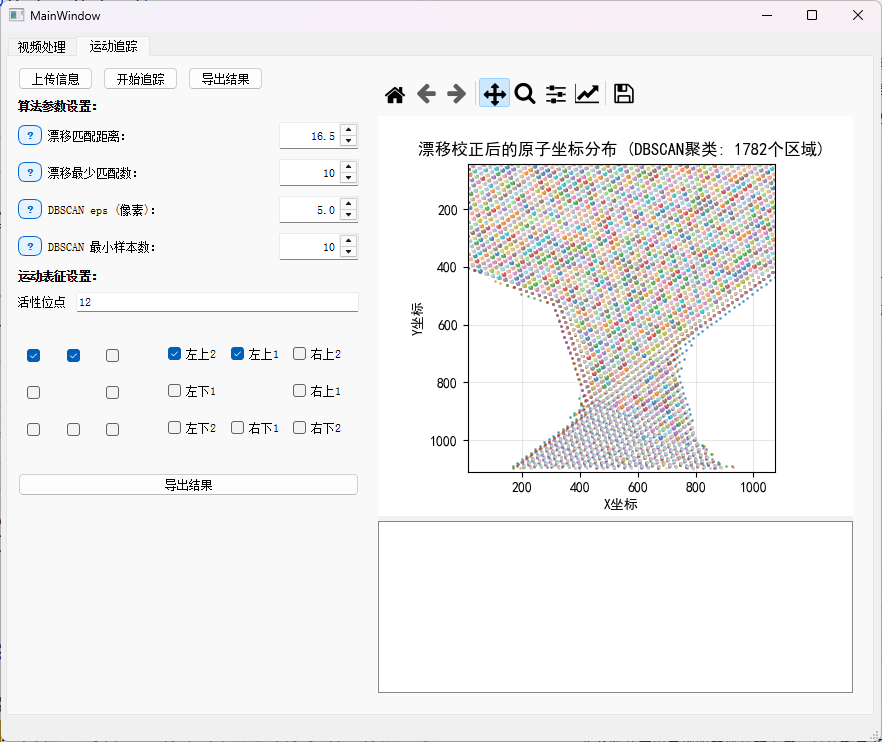
\includegraphics[width=0.6\textwidth]{images/chap5/运动追踪.png}
    \bicaption{运动追踪}{Motion Tracking}
    \label{fig:5-12}
\end{figure}

系统提供三类交互功能，第一类是平移视图，通过使用工具栏的平移工具拖动视图；第二类是缩放视图，通过使用工具栏进行缩放或者使用鼠标滚轮进行缩放；第三类是查看轨迹信息，可以点击可视化图中的任意圆圈，圆圈会高亮显示（变为红色粗线），在圆圈附近显示该原子在第一帧中的原始ID，如图\ref{fig:5-13}显示ID为1085，下方表格显示了该原子在所导入的所有帧中的详细信息，包括该点到各个邻接点之间的距离和所形成的角度。

\begin{figure} [htb]
    \centering
    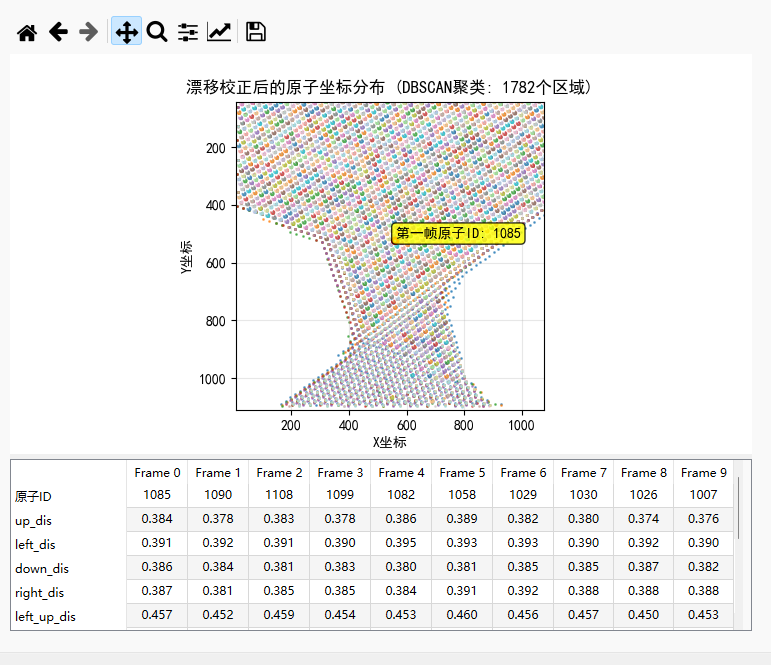
\includegraphics[width=0.6\textwidth]{images/chap5/轨迹信息.png}
    \bicaption{轨迹信息}{Trajectory Information}
    \label{fig:5-13}
\end{figure}

\section{本章小结}
本章设计并实现了一个高分辨TEM图像自动表征系统，主要包括自动化原子位置识别与处理模块和原子细粒度信息动态提取模块。系统通过前后端分离的Web架构，结合Node.js、Vue3、Python和PyTorch等技术，实现了高效的图像处理、原子定位、关系建模以及动态追踪功能。用户可以通过系统上传高分辨TEM图像和视频数据，进行预处理、原子位置识别、关系建模以及动态追踪分析，并通过可视化工具直观展示分析结果。系统还支持数据导出功能，为科学家们提供了强大的工具来深入分析材料的结构和性能，为后续的科学研究提供了重要的数据支持和分析手段。